\chapter{Xây dựng và triển khai hệ thống}
\label{ch:xay-dung}

\section{Môi trường phát triển}

Hệ thống được phát triển trên Windows với Python 3.x trong môi trường ảo (\texttt{.venv}), quản lý mã bằng Git. Kiểm thử dùng \texttt{pytest}; script PowerShell hỗ trợ verify phase. Không phụ thuộc dịch vụ LLM trực tuyến trong đường đánh giá lab.

\section{Công nghệ và công cụ sử dụng}

\begin{table}[H]
\centering
\caption{Công nghệ và công cụ chính}
\label{tab:tech}
\begin{tabular}{@{}p{0.28\linewidth}p{0.62\linewidth}@{}}
\toprule
\textbf{Thành phần} & \textbf{Lựa chọn} \\
\midrule
Ngôn ngữ & Python 3 \\
API gateway & FastAPI / Starlette \\
Lưu trữ truy hồi & SQLite FTS5, xếp hạng BM25 \\
Tối ưu truy hồi ngữ nghĩa & \texttt{numpy} (nhân ma trận), embedding cục bộ, vector \texttt{float32} lưu BLOB \\
Kiểm soát truy cập & RBAC theo vai trò/phòng ban (ACL trước truy hồi) \\
LLM lab & Mock Provider tất định; tuỳ chọn mô hình cục bộ (Semantic Judge) \\
Kiểm thử & pytest \\
Đóng gói phát hành & ZIP chuẩn, SHA-256, hard link publish \\
Tài liệu & Markdown + LaTeX báo cáo \\
\bottomrule
\end{tabular}
\end{table}

\section{Tổ chức mã nguồn}

Mã nguồn nhóm thành: \texttt{app/} (gateway, guards, RAG); \texttt{scripts/} (đánh giá, verify phase, release); \texttt{tests/}; \texttt{datasets/v2/} (benchmark đóng băng); \texttt{release/} (chính sách); \texttt{docs/}. Thư mục evidence/holdout không nằm trong gói phát hành chuẩn.

\section{Xây dựng chuỗi guard phòng thủ}

Chuỗi guard được hiện thực thành các module độc lập trong \texttt{app/guards/},
mỗi module trả về quyết định trong tập \{Allow, Block, Sanitize, Human-review,
Log\} theo thứ tự mức độ nghiêm trọng cố định (\emph{fail-closed}: quyết định
nghiêm khắc nhất thắng).

\begin{itemize}
    \item \textbf{Input Guard:} tập luật regex phát hiện prompt injection trực
    tiếp, jailbreak và ghi đè chỉ thị; chuẩn hoá văn bản (khoảng trắng, ký tự
    ẩn, biến thể chữ) trước khi đối chiếu để giảm né tránh.
    \item \textbf{RAG Context Guard:} đối chiếu luật trên \emph{ngữ cảnh truy
    hồi}, phát hiện chỉ thị ẩn trong bình luận HTML, tài liệu mạo danh thẩm
    quyền và mẫu poisoning; hỗ trợ làm sạch (sanitize) từng đoạn.
    \item \textbf{Output Guard / DLP:} rà mẫu bí mật (khoá API, token) và thông
    tin nhạy cảm trên phản hồi trước khi trả về; fail-closed khi vi phạm rõ.
    \item \textbf{Semantic Judge:} tuỳ chọn, gọi một mô hình ngôn ngữ cục bộ
    phán đoán ý đồ với các đòn tấn công ngữ nghĩa mà luật bỏ lọt.
\end{itemize}

\section{Xây dựng cơ chế truy hồi vectorized}

Cơ chế truy hồi lai kết hợp BM25 (SQLite FTS5) với xếp hạng ngữ nghĩa. Để giảm
độ trễ khi kho tài liệu lớn, vector embedding được chuẩn hoá đơn vị và lưu dưới
dạng khối \texttt{float32} (BLOB) trong SQLite; khi truy vấn, toàn bộ ma trận
vector được đọc trực tiếp và chấm điểm bằng \emph{một} phép nhân ma trận
\texttt{numpy} (tích vô hướng chính là cosine do vector đã chuẩn hoá), thay cho
vòng lặp Python và phân tích JSON trên từng tài liệu. Hai danh sách xếp hạng
được hợp nhất bằng Reciprocal Rank Fusion.

Kiểm soát truy cập (RBAC) được áp \emph{trước} bước truy hồi: mỗi tài liệu mang
vai trò/phòng ban và mức nhạy cảm; người dùng chỉ truy hồi được tài liệu trong
phạm vi quyền, độc lập với các guard nội dung.

\begin{figure}[H]
\centering
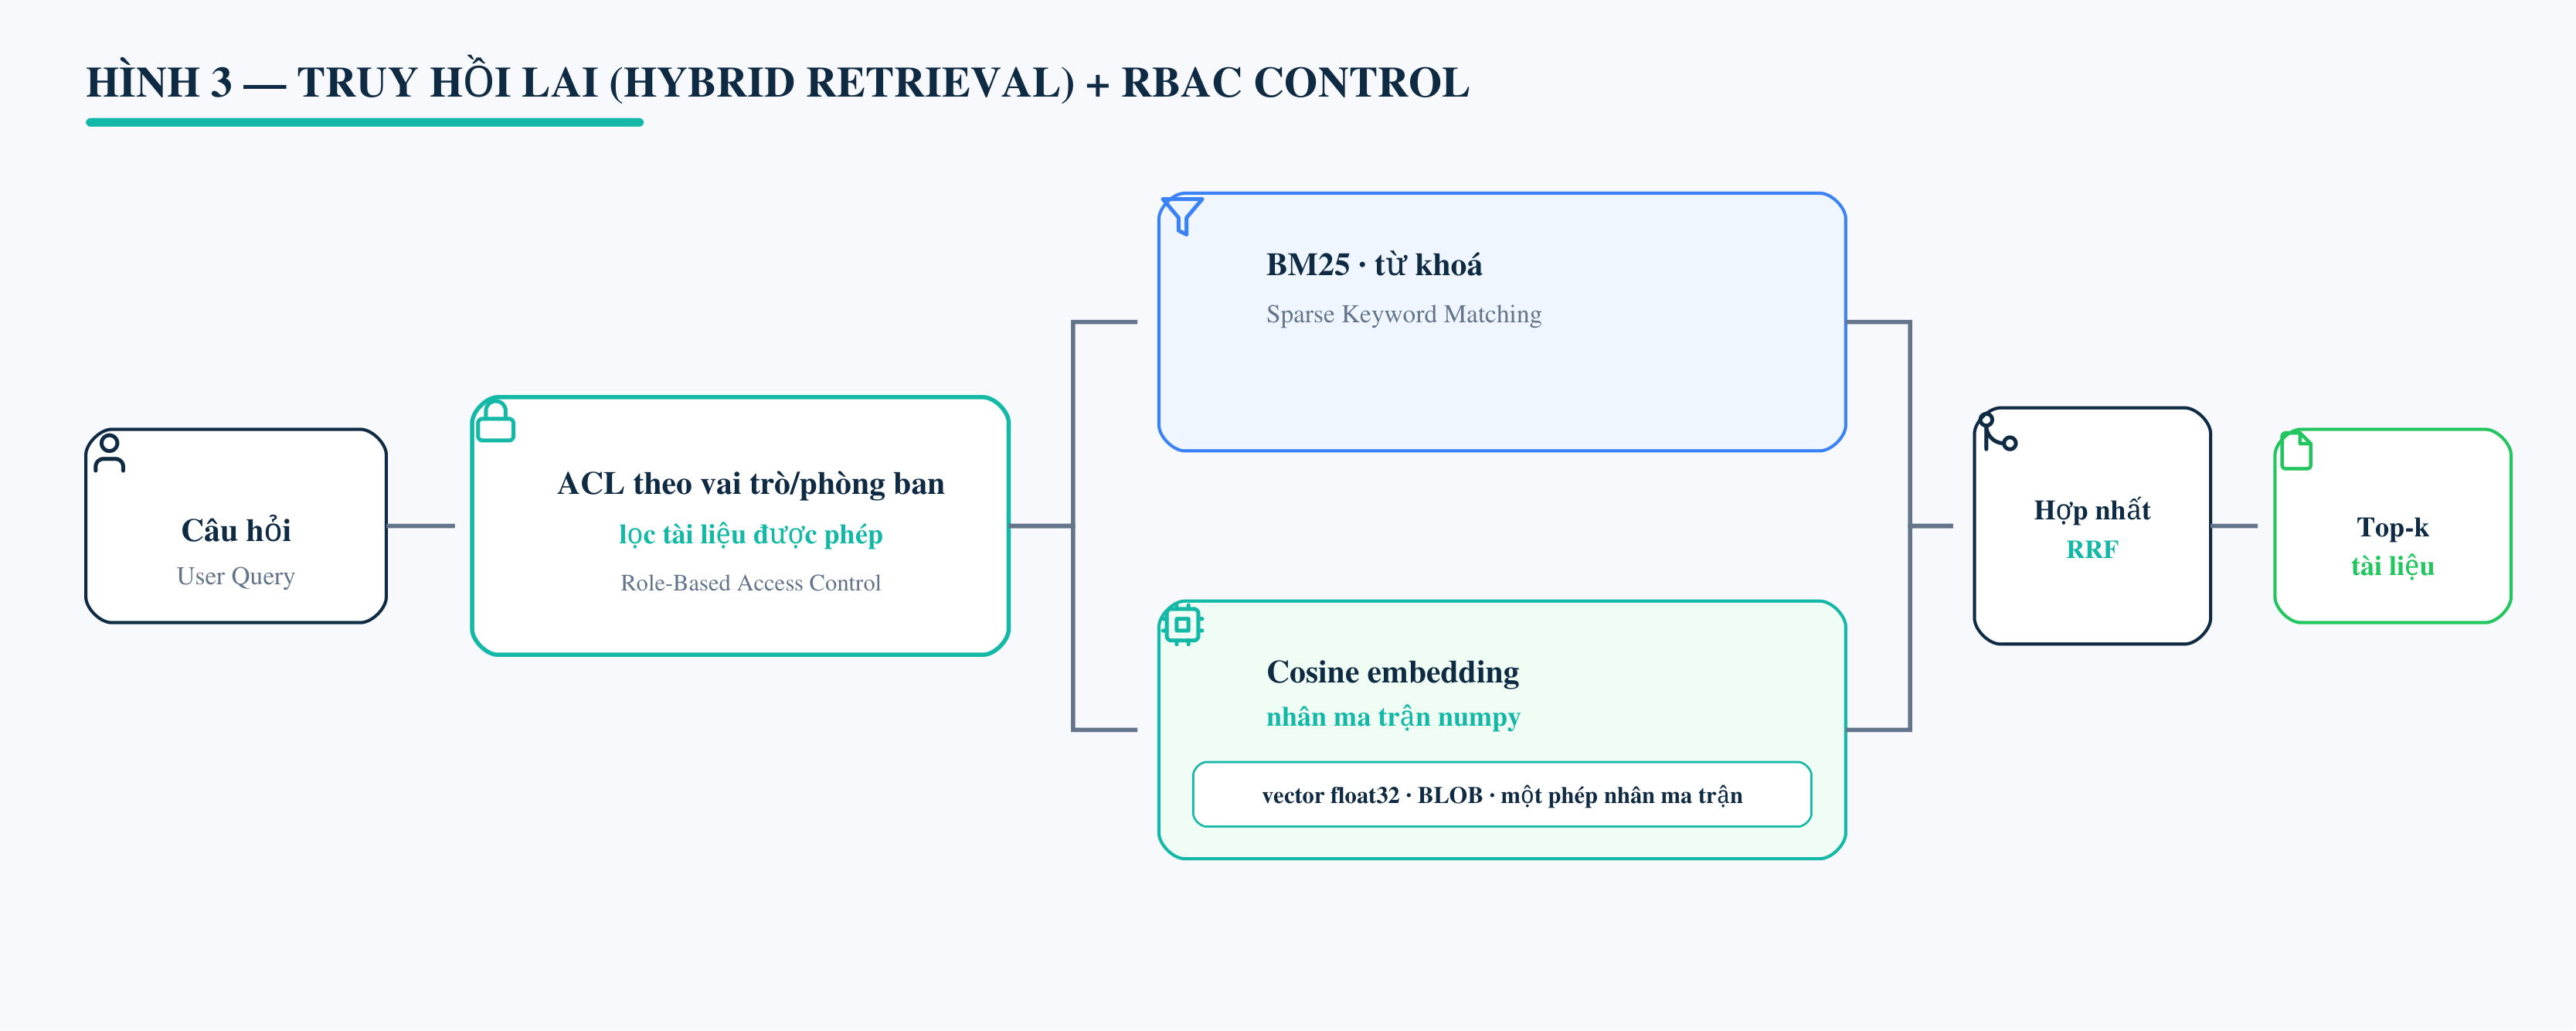
\includegraphics[width=\linewidth]{figures/fig-rag-rbac.png}
\caption{Cơ chế truy hồi lai (BM25 + embedding) kết hợp kiểm soát truy cập RBAC}
\label{fig:rag-rbac}
\end{figure}

Hình~\ref{fig:rag-rbac} minh hoạ luồng: câu hỏi trước hết qua bộ lọc ACL theo
vai trò/phòng ban, sau đó được chấm điểm song song bằng BM25 (từ khoá) và cosine
embedding (nhân ma trận trên vector \texttt{float32}), rồi hai danh sách được hợp
nhất bằng Reciprocal Rank Fusion để chọn ra tài liệu liên quan nhất.

\section{Xây dựng cơ chế quản lý chính sách}

Chính sách release-allowlist dùng schema cố định (phiên bản 4 trong gói đã rà soát). Mỗi đường dẫn được phân loại bằng đếm số rule khớp; overlap hoặc không khớp đều fail-closed. Policy được neo từ file ngoài khi verify để PASS.

\section{Xây dựng cơ chế ảnh chụp dữ liệu tin cậy bất biến}

Builder đọc policy (và declaration generated nếu có) một lần thành snapshot bất biến; cùng object snapshot dùng cho verify trước và sau publish, tránh đường tin cậy bị sửa giữa chừng.

\section{Xây dựng bộ kiểm tra gói phát hành}

\subsection{Kiểm tra manifest}
Đối chiếu schema, counts, control coverage, identity policy nhúng với neo tin cậy.

\subsection{Kiểm tra checksum và kích thước}
Tập khóa \texttt{FILE\_SIZES} và \texttt{SHA256SUMS} phải khớp tập payload/control đã định nghĩa; băm từng entry được tính lại.

\subsection{Kiểm tra cấu trúc ZIP}
Local records liên tục từ offset 0 đến central directory; EOCD tại EOF; không ZIP64; không byte thừa; comment ngoài rỗng; timestamp local/central thống nhất.

\subsection{Kiểm tra đường dẫn đa nền tảng}
Validator dùng chung từ chối ký tự/drive/ADS/UNC/traversal/tên dành riêng.

\subsection{Kiểm tra archive lồng nhau}
Chỉ kiểm tên/metadata thành viên; không giải nén nội dung tùy ý ra đĩa trong quy trình verify chuẩn.

\section{Xây dựng cơ chế xuất kết quả an toàn}

\subsection{Kết quả PASS}
Chỉ khi neo policy ngoài khớp và mọi kiểm tra đạt; exit 0.

\subsection{Kết quả FAIL}
Cấu trúc/ứng viên không hợp lệ hoặc vi phạm chính sách; exit 1.

\subsection{Kết quả NOT\_VERIFIABLE}
Thiếu neo đủ mạnh (ví dụ chỉ có hash policy); exit 2; không bao giờ được coi là PASS.

\subsection{Cơ chế ghi tệp nguyên tử}
Ghi temp cùng thư mục, flush/fsync, rồi thay thế nguyên tử; thành công thì không nhân bản ra terminal khi đã chọn file sink.

\subsection{Xử lý lỗi đầu ra}
Lỗi ghi/stream $\Rightarrow$ fallback content-free cố định, exit khác 0; không giữ PASS/partial; double-stream failure không ném traceback công khai.

\section{Cơ chế xác minh trước khi phát hành}

Builder dựng ZIP trên staging, chạy verifier đạt PASS, mới publish. Thất bại pre-publish không để lại thư mục đích hoàn chỉnh.

\section{Cơ chế phát hành không ghi đè}

Publish candidate dùng hard link no-clobber (\texttt{os.link}); không \texttt{os.replace} cho ZIP ứng viên; đích đã tồn tại thì fail. Các thư mục candidate lịch sử được giữ nguyên, không ghi đè.

\section{Tích hợp kiểm thử tự động}

Bộ test release/CI chạy trên fixture tổng hợp; kiểm thử inject lỗi ghi file, argparse độc hại, ZIP hỏng. Full suite lab ghi nhận hàng nghìn case đạt (Chi tiết Chương~4).

\section{Kết luận chương}

Hệ thống lab gồm runtime guard/RAG và lớp release-assurance đã được hiện thực theo nguyên tắc fail-closed, content-free và tái lập. Chương~4 trình bày phương pháp và kết quả kiểm thử.
